\documentclass{article}
\usepackage[english]{babel}
\usepackage[letterpaper,top=2cm,bottom=2cm,left=3cm,right=3cm,marginparwidth=1.75cm]{geometry}
\usepackage{amsmath}
\usepackage{graphicx}
\usepackage[colorlinks=true, allcolors=blue]{hyperref}
\title{An effective solution to the symmetric travelling salesman problem using genetic algorithms is to find the shortest route among a large number of possible routes for a school bus to travel at the lowest feasible cost (distance).}
\date{March, 2022}
\author{ Midnapore college (Autonomous) \\ Depertment of Computer Science \\ Guide : Prof. Shovan Roy (Department of CSA \\ Group : Suman Paik | Arun Sarma | Rohan Das | Sumit Mondal
% \and Richard Row, \LaTeX\ Academy
}

\begin{document}
\maketitle
\noindent
\rule{\textwidth}{0.5pt}

\vspace{0.1cm}\textbf{Abstract  } The Travelling Salesman Problem is a classical combinatorial optimization problem, which is a simple concept but it is very difficult to solve. A TSP case like, there are many routes that are interconnected to each other that can be multiple routes or a single route within two cities and people get confused to decide which route is the best choice for them to travel through the all cities that contains the minimum cost. School bus route problem is this type of problem. Here we need two things such as time and fuel efficiency. That means the only condition among all the routes is which route will be the best choice for travelling through those cities with minimum distance so that we can get the maximum benefit from it like minimum distance or minimise time and better fuel efficiency. When the routes are massive in number then this kind of complex problem arises. So in this TSP type problem we can't find the best route because the probability of tours within the cities are huge. In this situation Genetic Algorithm gives us the power to solve this kind of problem. Researchers  are continuously trying to solve this problem through various methods, Genetic Algorithm is one of them. Here we present a 2D, 3D, 4D Travelling Salesman problem where there can exist multiple or single routes between two cities but the main one thing is there is no sub tour between those cities, every tour is independent that means each route covers all cities but repetition is not considered. Some genetic properties or concepts like crossover and mutation operators are used for solving the problem and we also show the experimental results in order to express the working model of the Genetic Algorithm.



\vspace{0.2cm}\textbf{Keywords  } Travelling salesman problem,2D,3D,4D model, symmetric TSP, Genetic algorithm, Crossover Mutation Operator,Fitness value Shortest root, Selection, Evolution.
\par\noindent\rule{\textwidth}{0.5pt}
\section{Introduction}
TSP is to find the shortest way of visiting each city exactly once and return to the start point. In the case of the
symmetric travelling salesman problem the distance between two cities is different when travelling in the opposite
direction, the costs may vary, at times only one-way traffic is allowed on the way from one city to another. Although
the statement is easy to say but more difficult to resolve. Travelling Salesman Problem is an optimization problem
and there is a vast search space, named NP-hard which means it cannot be solved in polynomial time. TSP is being
applied in many cases such as microchip making, vehicle routing, drilling on printed circuit boards, Overhauling gas
turbine engines etc. let’s say we have a set of numbers of n cities, and then we can get (n - 1)! alternative routes to
cover all n cities. With the help of TSP, we can find the shortest path.
\section{Literature review}
\quad \quad The Travelling Salesman problem has a basic concept, however it is more complex to solve. The Travelling Salesman Problem is an optimization problem with a large search space that is NP-hard, meaning it cannot be solved in polynomial time. It is currently one of the most essential issues in the field of computer science. Researchers have combined the Genetic Algorithm techniques with the Travelling Salesman Problem (TSP) to solve this type of issue in polynomial time. We present crossover and mutation operators to solve this kind of problem and they also express the experimental results obtained with different standard examples using combinations of crossover and mutation operators in relation with path Representation. \\
\par
While computer models of evolutionary processes date back to the 1950s, John Holland invented most of what we now call genetic algorithms (also known as "GAs"). He is the professor at the University of Michigan, whose book Adaptation in Natural and Artificial Systems pioneered GA research. Nowadays the genetic algorithm is a part of a wider field of research, often referred to as "Evolutionary Computing." In computer science and operations research, a Genetic Algorithm (GA) is a metaheuristic that belongs to the larger class of evolutionary algorithms and is inspired by natural selection (EA). To develop high-quality solutions to optimization and search problems, genetic algorithms use biologically inspired operators such as mutation, crossover, and selection. Researchers are continuously trying to improve the Genetic Algorithm methods or the single operators for improving the overall performance of this algorithm. \\
\par
The researchers are continuously trying to find a better way to solve the TSP problem with the help of Genetic Algorithm. There is an exciting review paper about the selection method of Genetic Algorithm which was used to get the result of Land Suitability [5]. In another case other researchers had worked on the topic of genetic algorithm which contain the different selection methods [3]. Researchers were trying to solve this TSP using different selection, crossover, mutation operators [1] [2]. There is an excellent book which can build the concept of genetic algorithm in a better way called “Introduction of Genetic Algorithm”[4].
\section{Travelling Salesman Problem}
The Travelling Salesman Problem is a NP-hard problem, meaning that no exact algorithm exists to solve this kind of
problem in polynomial time. The predicted time to find the best solution is exponential.The shortest path problem is
characterised as a combinatorial problem with the goal of finding the shortest path (or the minimum cost). Cities are
the graph's vertices, pathways are the graph's edges, and a path's distance is the edge's length, hence TSP can be
represented as an unsupervised weighted graph. It's a minimization issue that starts and ends at a certain vertex after only visiting each other vertex once. [2]

\subsection{Classical TSP Model}
TSP can be written as graph G = (V, E) in a classical two-dimensional TSP, where V = 1, 2,..., N is the set of nodes,
and E is the set of edges. A salesman has to travel to N cities at minimum cost. In this tour, the salesman begins in
one location, visits each city exactly once, and then returns to the beginning city at minimum cost. Let $C_{ij}$ represent
the cost of travel from the i-th city to j-th city. Then the model is mathematically formulated as
\[
\quad \textrm{Determine a complete tour}\quad x_{ij},i=(1,2,...,N),j=(1,2,...,N)
\]
\[
\quad \textrm{to minimize}\quad Z=\sum^{N-1}_{i=1}\sum^{N-1}_{j=1}x_{ij}c_{ij},
\]
\[
\quad \textrm{subject to}\quad Z=\sum^{N-1}_{i=1}x_{ij}=1,\quad \sum^{N-1}_{j=1}x_{ij}=1
\]
\[
\sum_{i\in s}\sum_{i\in s}x_{ij}\le \quad \mid S \mid - 1, \forall S \subset V 
\]

\subsection*{Classical TSP with time for minimum total travel time Model}
Let $t_{ij}$ be the time for travelling from i-th city to j-th city. Following this model is formulated as
\[
\quad \textrm{Determine a complete tour}\quad(x_1,x_2,...,x_N,x_1)
\]
\[
\quad \textrm{minimize}\quad Z=\sum^{N-1}_{i=1} t_{x_i,x{i+1}}+t_{x_N,x_1}
\]

\subsection{3D TSP Model}
Let us consider c(i, j, r) and t(i, j, r) be the cost and time respectively for travelling from i-th city to j-th city by the r-th
route. Now the salesman has to determine a complete tour ($x_1$, $x_2$,..., $x_N$ , $x_1$) and
corresponding available route types ($r_1$, $r_2$, ..., $r_s$ ).$r_i$ $\in$ $\{1, 2, ..s$\}. The problem can be expressed mathematically as:
\[
\quad \textrm{minimize}\quad Z =\sum^{N-1}_{i=1} c(x_i,x_{i+1},r_i)+c(x_N,x_1,r_1), \] 
\[ \quad \textrm{subject to}\quad\sum^{N-1}_{i=1} t(x_i,x_{i+1},r_i),\]
\[
\quad \textrm{where}\quad x_i \ne x_j,i,j=1,2,...N,\quad \textrm{}\quad r_i,r_1 \in 1,2,..ors) 
\]
\subsection{4D TSP Model}
Let us consider c(i, j, r, k) and t(i, j, r, k) be the cost and time respectively for travelling from i-th city to j-th city by the r-th
route using k-th type conveyance. Then the salesman has to determine a complete tour ($x_1$, $x_2$,..., $x_N$ , $x_1$) and
corresponding available route types ($r_1$, $r_2$, ..., $r_s$ ) with conveyance types ($v_1$, $v_2$, ..., $v_p$ ) to be used for the tour,
where $v_i$ $\in$ {1,2, ..N} for i = 1, 2, ..., N, $r_i$ $\in$ $\{1, 2, ..s$\} and $v_i$ $\in$ $\{1,2, ..p$\} for i = 1,2, ..., N and
all $x_i$'s are distinct. The problem can be expressed mathematically as:
\[
\quad \textrm{minimize}\quad Z =\sum^{N-1}_{i=1} c(x_i,x_{i+1},r_i,v_i)+c(x_N,x_1,r_1,v_1), \] 
\[ \quad \textrm{subject to}\quad\sum^{N-1}_{i=1} t(x_i,x_{i+1},r_i,v_i)+t(x_N,x_1,r_1,v_1)\leq t_{max},\]
\[
\quad \textrm{where}\quad x_i \ne x_j,i,j=1,2,...N,\quad \textrm{}\quad r_i,r_1 \in 1,2,..ors),\quad v_i,v_1 \in (1,2,..orp)
\]

\section{Genetic Algorithm}
A genetic algorithm is a heuristic search algorithm used to solve search and optimization problems. This algorithm
can solve problems very fast which if you try to solve by brute force that would take too much time for it. This
algorithm can be used in many real-life applications such as data centres, image processing, codebreaking,
electronic circuit design, and artificial creativity. Genetic algorithms are inspired by the concept of genetics and
natural selection to provide best solutions to problems. GA is based on the behaviour of chromosomes and their
genetic structure. Here each chromosome participates with a vital role to produce the possible solutions. Here the
fitness function is used to provide the characteristics of all individuals in the whole population. When the function is
bigger then the solution is much more accurate. That's why these algorithms have better intelligence than random
search algorithms because these algorithms use historical data to take the search to the best performing region within
the solution space[4].
\begin{center}
    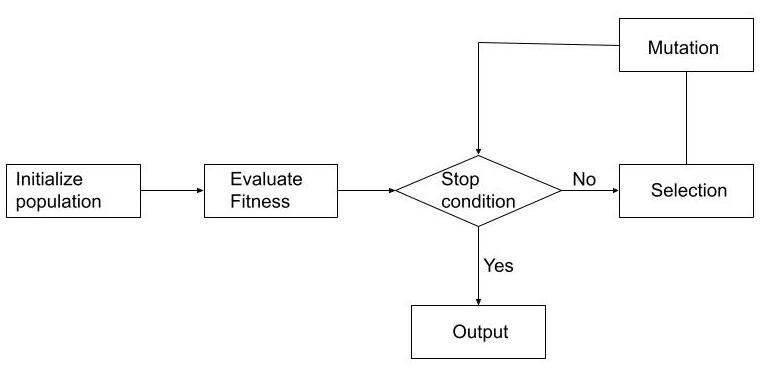
\includegraphics[width=12cm]{Untitled drawing (1).jpg}
\end{center}

\section{Genetic Algorithm follow the following phases to solve complex optimization problems}
To begin, the genetic algorithm creates an initial population. All possible solutions to the given problem are included
in this initial population. The usage of random binary strings is the most common method for initialization.
\subsection{Fitness assignment}
The fitness function assists in determining the fitness of the entire population. Every
individual is given a fitness score, which determines their chances of being picked for reproduction. The better the
fitness score, the more likely you are to be selected for reproduction.
\subsection{Selection Strategy for Reproduction}
To improve reproduction, the selected individuals are grouped in pairs of
two. The genes of these people are passed down to the following generation. The major goal of this phase is to
identify the region with the best probability of coming up with the best solution to the problem (better than the
previous generation). The fitness proportionate selection strategy is utilised by the genetic algorithm to ensure that
useful recombination solutions are used. The selection operator ensures the better members of the population (with
higher fitness) so that the better members can reach the next generation. So there are various kinds of selection
strategies. Some popular methods are given below.
\subsubsection{Tournament Selection}
Tournament Selection is one of the most popular selection methods in genetic algorithms. In this method the chance
of selecting individuals are performed based on their fitness values. The primary idea behind this technique is to select the individual with the highest fitness value from a particular number of chromosomes in the population into
the next generation. There is no arithmetical computation based on fitness value in the tournament selection, only a
comparison between individuals based on fitness value. Here Tournament size refers to the number of chromosomes
that will be competing in the tournament. This technique is faster than the roulette wheel and Rank Based selection
method[3].
\subsubsection*{\textbf{Algorithm}}
\begin{enumerate}
    \item We select the tournament size n at random.
    \item We pick n individuals from the population, at random and determine the best one in terms of their fitness values.
    \item The best individual is copied into the mating pool.
    \item Thus, in this scheme only one individual is selected per tournament and $N_p$ tournaments are to be played to make the size of the mating pool equal to $N_p$
\end{enumerate}
\subsubsubsection{\textbf{Pseudocode}}
\\While population size < popsize do \\
  Generate popsize random number r \\
  Calculate cumulative fitness, total fitness ( $p_i$ ) and sum of proportional fitness (Sum)
 \\
  If Sum <r then \\
  Select the first chromosome \\
  End If \\
  End While \\
  Retum chromosomes with fitness value \\ 
  End Procedure [3] \\
  
\subsubsubsection{\textbf{Input}} 
A Population of size N with their fitness values Output: A mating pool of size $N_p$ ($N_p$ $\le$ N) 
Steps: 1) Select $N_u$ individuals at random ($N_u$ $\le$ N). 2)Out of $N_u$ individuals, choose the individual with the highest fitness value as the winner. 3) Add the winner to the mating pool, which is initially empty. 4) Repeat Steps 1-3 until the mating pool contains $N_p$, individuals 5) Stop
Example of Tournament Selection method : Here, N = 8, $N_u$ = 2, $N_p$ = 8 

\begin{center}
\begin{tabular}{|l|l|l|l|l|l|l|l|l|} 
\hline
\textbf{Individual} & 1                                                & 2                                                & 3                                                & 4                                                & 5                                                & 6                                                & 7                                                & 8                                                 \\ 
\hline
\textbf{Fitness}    & \textcolor[rgb]{0.263,0.263,0.263}{\textbf{2.0}} & \textcolor[rgb]{0.263,0.263,0.263}{\textbf{3.1}} & \textcolor[rgb]{0.263,0.263,0.263}{\textbf{4.1}} & \textcolor[rgb]{0.263,0.263,0.263}{\textbf{5.0}} & \textcolor[rgb]{0.263,0.263,0.263}{\textbf{5.6}} & \textcolor[rgb]{0.263,0.263,0.263}{\textbf{2.9}} & \textcolor[rgb]{0.263,0.263,0.263}{\textbf{2.8}} & \textcolor[rgb]{0.263,0.263,0.263}{\textbf{5.5}}  \\
\hline
\end{tabular}
\end{center}
\begin{center}
\subsubsubsection{\textbf{Output}} \\
\begin{tabular}{|l|l|l|} 
\hline
$N_u$ trial individual                                                                                                                                                                                                                                                                                                                                            & Individual pair                                                                                                                                                                                                                                                                                                                                                                & Selected Individua\textcolor[rgb]{0.263,0.263,0.263}{l}                                                                                                                                                                                                                                                                                                         \\ 
\hline
\begin{tabular}[c]{@{}l@{}}\textcolor[rgb]{0.263,0.263,0.263}{1}\\\textcolor[rgb]{0.263,0.263,0.263}{2}\\\textcolor[rgb]{0.263,0.263,0.263}{3}\\\textcolor[rgb]{0.263,0.263,0.263}{4}\\\textcolor[rgb]{0.263,0.263,0.263}{5}\\\textcolor[rgb]{0.263,0.263,0.263}{6}\\\textcolor[rgb]{0.263,0.263,0.263}{7}\\\textcolor[rgb]{0.263,0.263,0.263}{8}\end{tabular} & \begin{tabular}[c]{@{}l@{}}\textcolor[rgb]{0.263,0.263,0.263}{2,4}\\\textcolor[rgb]{0.263,0.263,0.263}{3,8}\\\textcolor[rgb]{0.263,0.263,0.263}{1,3}\\\textcolor[rgb]{0.263,0.263,0.263}{4,5}\\\textcolor[rgb]{0.263,0.263,0.263}{1,6}\\\textcolor[rgb]{0.263,0.263,0.263}{1,2}\\\textcolor[rgb]{0.263,0.263,0.263}{4,2}\\\textcolor[rgb]{0.263,0.263,0.263}{8,3}\end{tabular} & \begin{tabular}[c]{@{}l@{}}\textcolor[rgb]{0.263,0.263,0.263}{4}\\\textcolor[rgb]{0.263,0.263,0.263}{8}\\\textcolor[rgb]{0.263,0.263,0.263}{3}\\\textcolor[rgb]{0.263,0.263,0.263}{5}\\\textcolor[rgb]{0.263,0.263,0.263}{6}\\\textcolor[rgb]{0.263,0.263,0.263}{2}\\\textcolor[rgb]{0.263,0.263,0.263}{4}\\\textcolor[rgb]{0.263,0.263,0.263}{8}\end{tabular}  \\
\hline
\end{tabular}
\end{center}

 
\subsubsection{Proportional Roulette Wheel Selection}
In this particular selection method individuals are selected with a probability that is directly proportional to their
fitness values that means an individual's selection corresponds to a section of a roulette wheel. The probabilities of
choosing a parent can be compared to spinning a roulette wheel, with the size of each section related to the parent's
fitness. Individuals with the largest fitness value have the higher probability of being selected. Within the roulette
wheel, the fittest individual occupies the largest segment, while the least fit occupies a smaller segment.The sum of
all the individuals' fitness values makes up the roulette wheel's circumference. When the wheel is spun, it will
eventually come to a halt, and the pointer attached to it will point at one of the segments, most likely the broadest.
All segments, on the other hand, have a chance, with a probability proportionate to their width. By repeating this
process each time an individual must be picked, the better individuals will be chosen more frequently than the
inferior ones, ensuring that the survival of the fittest conditions are met. Let’s consider f1, f2,…, f n are the fitness
values of the individuals 1, 2,…, n. Selection probability ( $P_i$ ) for individual i is -    
\[ 
P_{i} = \frac{f_i}{\sum^{n}_{j=1} f_j}
\]
The primary benefit of proportional roulette wheel selection is that it does not dismiss any individuals from the
population and allows all of them to be chosen. As a result, population diversity is preserved. However, there are a
few key flaws in proportional roulette wheel selection. Outstanding individuals will represent bias at the start of the
search, which could lead to an early convergence and loss of diversity. If an early population includes one or two
very fit but not the best individuals, and the remainder of the population is poor, these fit individuals will quickly
dominate the population, preventing the population from exploring other potentially better individuals.Such a great
domination results in a significant loss of genetic variety, which is unfavourable to the optimization process.


\subsubsubsection{\textbf{\\ Procedure:}}
\\While population size < popsize do\\
Generate popsize random number r\\
Calculate cumulative fitness, total fitness ( $P_i$ ) and sum of proportional fitness (Sum)\\
Spin the wheel popsize times\\
If Sum $<$ r then\\
Select the first chromosome, otherwise. select j-th chromosome\\
End If\\
End While\\
Return chromosomes with fitness value proportional to the size of selected wheel section\\
End Procedure [3]

  
\subsubsection{Rank-based selection}
Rank-based selection is a selection method in which a chromosome's probability of being chosen is determined by
its fitness rank in comparison to the overall population. Rank-based selection first sort the individuals in the
population based on their fitness before computing selection probabilities based on their ranks rather than fitness
values whereas the proportional Roulette wheel selection considers the fitness value and computes probability based
on it and the best individual heavily dominates the entire population, resulting in a significant loss of genetic variety,
which is not beneficial to the optimization process. This is one of the biggest problems of the roulette wheel
selection.To overcome this problem with Roulette-Wheel selection, a rank-based selection scheme has been
proposed. The process in rank selection consists of two steps. 1. The fitness values of the individuals are displayed
in increasing order. The individual, which has the lowest value of fitness is assigned rank 1, and other individuals
are ranked accordingly. 2. The proportionate based selection scheme is then followed based on the assigned rank[4].
The % area to be occupied by a particular individual i, is given by-
\[ 
\frac{R_i}{\sum^{n}_{i=1} R_i}
\]
Where Ri indicates the rank of the i - individual. The rank of two or more people with the same fitness values should
be the same. Rank-based Selection Example : There are 4 individuals and their fitness values are given below f1 =
0.40, f2 = 0.05, f3 = 0.03, f4 = 0.02. Their proportionate areas on the wheel are :  80 \%, 10 \%, 6 \%, and 4 \%

\begin{center}
\begin{tabular}{|l|l|l|l|l|} 
\hline
~ ~ Individual~ (i) & ~ ~ Fitness~ () & ~ ~ RW~ (Area) & ~ ~ ~ Rank & ~ ~ ~ RS~ (Area)  \\ 
\hline
~ ~ ~ ~ 1           & 0.60            & 80\%           & ~ ~ ~ 4    & 40\%              \\ 
\hline
~ ~ ~ ~ 2           & 0.07            & 10\%           & ~ ~ ~ 3    & 30\%              \\ 
\hline
~ ~ ~ ~ 3           & 0.05            & 6\%            & ~ ~ ~ 2    & 20\%              \\ 
\hline
~ ~ ~ ~ 4           & 0.02            & 4\%            & ~ ~ ~ 1    & 10\%              \\
\hline
\end{tabular}
\end{center}
\subsubsubsection{\textbf{Procedure:}}
\\While population size <popsize do
Sort population according to rank\\
Assign fimesses to the individuals according to linear rank function\\
Generate popsize random number (r)\\
Calculate cumulative fitness, total fitness and sum of proportional fitness (Sum)\\
Spin the wheel popsize times\\
If Sun $<$ r then\\
Select the first chromosome, otherwise, select j-th chromosome\\
EndIf\\
End While\\
Retum chromosomes with fitness value proportional to the size of selected wheel section\\
End Procedure\\
This is how the rank-based selection method overcomes the drawback of proportional roulette wheel selection without loss of genetic diversity.
\subsubsection{Probabilistic Selection}
For a minimum cost objective, it is better to choose that population which is in the neighborhood of the minimum
solution of the entire solution space. So we get the convergence rate much higher. From the initial population,
choose the best fitted population for TSP. It is chosen as the minimum fitness value (say f min ). To form the matting
pool, we use the Boltzmann-Probability of each chromosome from the initial population.
\[
\quad \textrm{Let,}\quad
P_B=e^{((f_{min}-f(x_i))/T)},
\]
\[
\quad \textrm{Where}\quad
T=t_{0(1-a)^k}, \quad k=(1+100)*(g/G)), 
\]
 g = current generation number, G = maximum generation, $T_0$ = rand[5,100],
a = rand[0,1], f($x_i$) means the chromosome corresponding to $x_i$, i = chromosome number.
\subsection{Crossover}
This operator swaps the genetic information of two parents to reproduce an offspring. It is
performed on parent pairs that are selected randomly to generate a child population of equal size as the parent
population.
Types of crossover Operator Crossover is one of the noticeable operators used in genetic algorithms. There are
various kind of crossover like -
\subsubsection{Order Crossover}
In this situation of order crossover, a piece of the first parent's chromosome gets copied to the offspring's
chromosome, and the offspring inherits the remaining values. Now select two cut points randomly in each parent's
genes.The consecutive alleles between two cut points from Parent 1 are copied to the Offspring 1. Then, the
remaining genes are copied from the second cut point in the order in which Parent 2 starts after the second cut point
till all positions are filled.
\subsubsection*{\textbf{Algorithm}}
The concept is to keep the pieces in their relative sequence.
Procedure: Informal
\begin{enumerate}
    \item Pick a random section from the first parent.
    \item Give the first child a copy of this section.
   
    \item To the first child,copy the numbers that 
     aren't in the first part
     \begin{itemize}
     \item {beginning at the duplicated part's cut point,}
     \item utilising the second parent's sequence,
     \item and wrapping around at the end
     \end{itemize}
    \item Reverse the parent roles for the second child [3]
\end{enumerate}
\begin{center}
    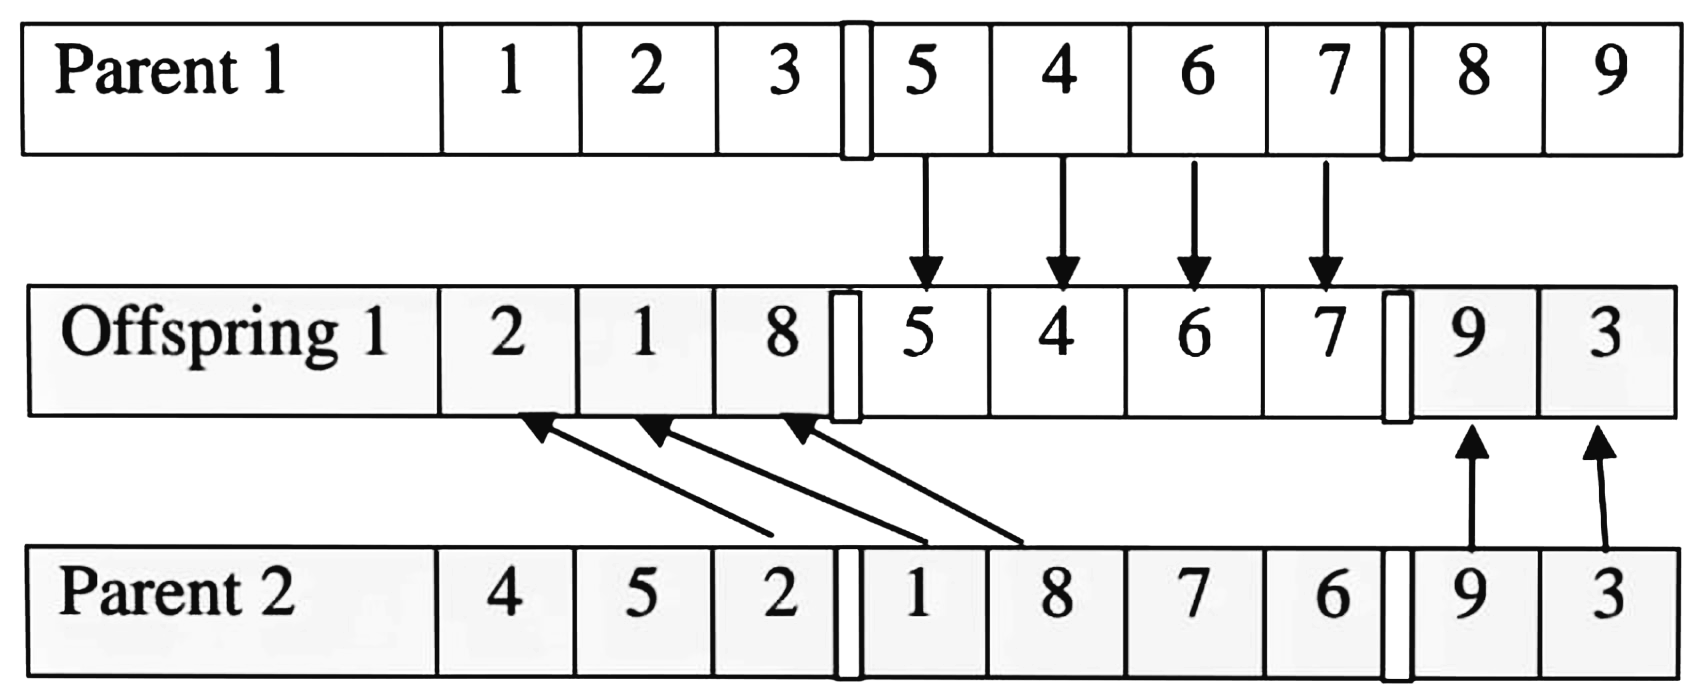
\includegraphics[width=8cm]{orderCrossover.png}
\end{center}

\subsubsection{Cyclic Crossover}
Generate a random number r from the range [0, 1] for each p(n) solution. If r $<$ $P_t$ then the solution is
taken for crossover.
% \subsubsection*{Crossover process}
\\
  \vspace{0cm}\textbf{Crossover process   }
The cyclic crossover procedure is used for simple TSP. The cyclic crossover focuses on subsets of cities that occupy
both parents in the same subset of positions. These cities are then copied from the first parent to the offspring, and
the remaining positions are filled with the cities of the second parent. As a result, each city's position is inherited
from one of the two parents. However, many edges can be broken in the process, because the initial subset of cities
is not necessarily located at consecutive positions in the parent tours.7\\
\\(1) Identify the gene in the first position of the second parent and go to the corresponding gene in the first parent.\\ (2)
Move vertically from the current gene of the first parent to the gene of the second parent.\\ (3) Check if the second
parent's gene is the same as the first parent's first gene. If yes, then go through step-(5); If not, then go through
step-4.\\ (4) Go to the first parent gene that corresponds to the current gene of the second parent and go to step-B.\\ (5)
Repeat the same steps to get the second offspring .\\ (6) Copy the genes present in the first parent cycle to the same
position as the first offspring. \\ (7) Copy the genes present in the second parent cycle to the same position as the
second offspring.\\(8) Copy the remaining genes of the second parent to the same position of the first offspring as
shown. \\(9) Copy the remaining genes of the first parent to the same position as the second offspring.\\ (10) The
current sequence of genes in each offspring forms the final similar offspring[4].
\begin{center}
    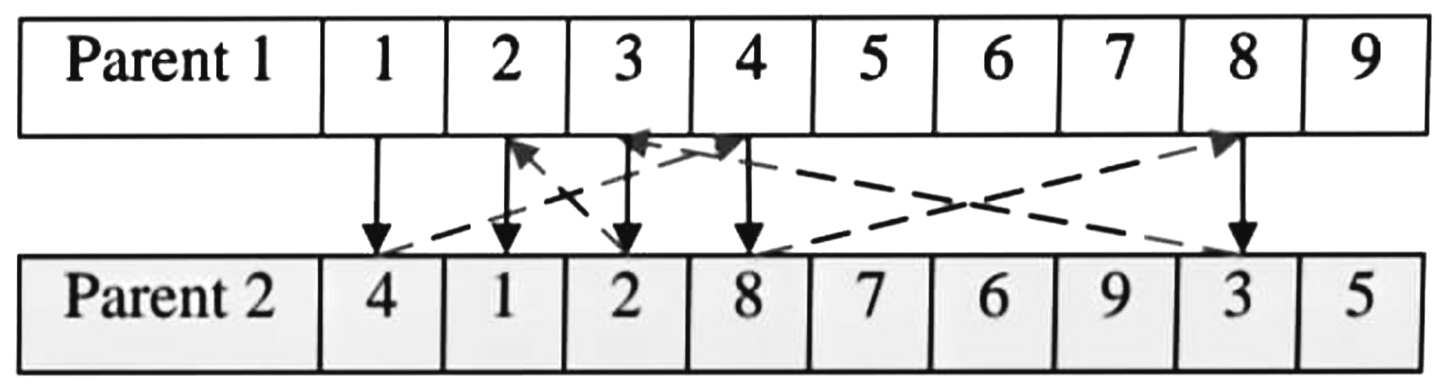
\includegraphics[width=8cm]{crossover01.png}
\end{center}
\begin{center}
     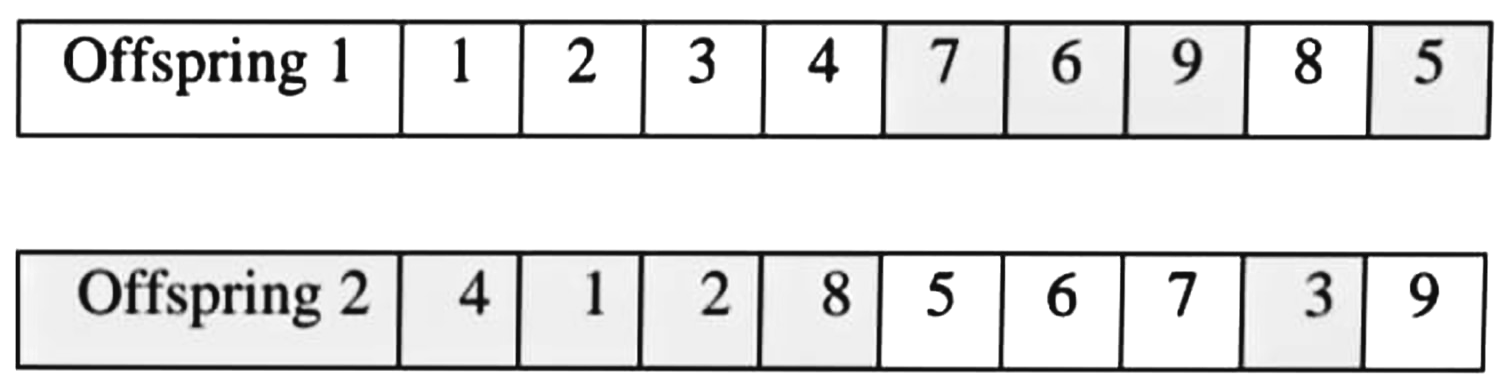
\includegraphics[width=8cm]{crossover02.png}
\end{center}
\subsubsection{Partially Mapped Crossover (PMX)}
PMX stands for partially matched crossover, and it works in a similar way to two-point crossover. Two crossover
points are chosen among two parents in this procedure, and the genes between the two crossover points are
exchanged, while the remaining genes are filled by partial mapping.
\begin{center}
    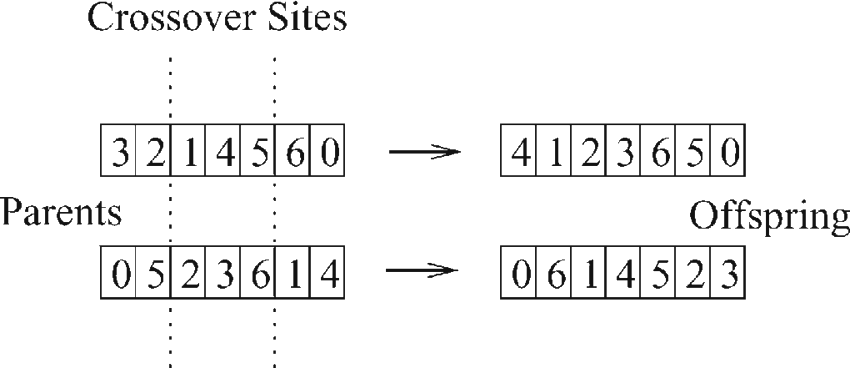
\includegraphics[width=8cm]{latexImage_ec81ff7afb5fadf70729ac7d59b20bbc.png}
\end{center}
\subsubsection{Multi-Parent Crossover}
Adaptation is a fairly popular topic in our culture nowadays as a result of various practical situations. Aside from the
original parents (father and mother), there are two additional parents (father and mother) who have been included. In
order to generate offspring, a new strategy with four parents (the first two are original parents and the other two are
adoptive parents) is used. This encouraged crossover approach selects four individuals or parents in an ergodic
manner to produce children. To obtain the best TSP results, we travel from one node to the next while keeping the
lowest possible travel cost depending on the TSP condition.
\subsection{Replacement}
Generational replacement, or the replacement of the old population with the new child population,
occurs during this phase. The new population has greater fitness scores than the previous population, indicating that
a better solution has been developed.
\subsection{Mutation}
This operator populates the new child population with new genetic information. This is achieved by flipping some
bits in the chromosome. Mutation solves the problem of local minimum and enhances diversification. The following
image shows how mutation is done.
\begin{center}
    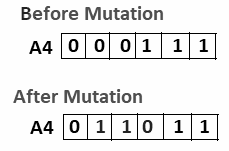
\includegraphics[width=4.5cm]{mutation01.png}
\end{center}
\subsubsubsection{Random Mutation}
Selection for mutation Generate a random number r from the range [0, 1] for each p(n) solution. If r $<$ $P_m$ then the
solution is used for mutation.
Mutation process
To mutate a TSP solution X = (x 1 , x 2 ,..., x N ) with T number of nodes, randomly select T number of nodes from the
solution and simply replace their positions in the solution, i.e., if two nodes x i , x j are randomly selected, then
interchange x i , x j to get a child solution. If the new solution satisfies the problem's constraint, it replaces the parent
solution. For CSTSP to mutate a solution (X,V), where X = (x 1 , x 2 ,..., x N ), at first an integer from the range [1, 2] is8
chosen randomly. If 1 is chosen, another two random integers i, j are selected in the range [1, N]. Then interchange
x i and x j to get a child solution. If the child solution satisfies the problem constraint, it replaces the parent solution.
\subsection{Termination}
After the replacement has been completed, a stopping criterion is utilised to determine when the project should be
terminated. When the threshold fitness solution is reached, the algorithm will stop. This answer will be identified as
the best in the population.



\subsection*{\hfil Conclusion \hfil}
In this literature we provide the overview of Genetic Algorithm as well as Travelling Salesman Problem. The travelling salesman problem(TSP) is an optimizationproblem which is very simple at the point of understanding. It seems Like a very simple task but it is very difficult to solve. The problem is to find the shortest path through a set of points or cities or Whatever you may like to say and the only condition is each city is visited exactly once. The problem is known as NP-hard, and cannot be solved in polynomial time when the points are so large in number. Many algorithms have been developed in this case. Here we use the Genetic Algorithm approach to solve this problem. Nowadays researchers are continuously trying to solve this kind of problem by improving this type of algorithm and try to find the cost minimally. So by using the researchers thought this is the approach of solving school bus routes like a type of TSP problem can be solved.


\subsection*{\hfil References \hfil}

\par[1] Genetic Algorithms for the Travelling Salesman Problem: A Review of Representations and Operators. January 1999, DOI:10.1023/A:1006529012972,Source DBLP. Pedro Larranaga-Universidad Politécnica de Madrid, Cindy Kuijpers-Tilburg University. \par[2] International Journal of Advanced Research in Computer Science and Software Engineering. Solving Travelling Salesman Problem Using Genetic Algorithm. Saloni Gupta, Poonam Panwar Department of Computer Science & Engineering Ambala College of Engineering & Applied Research, Ambala-133101, India\par[3]  Genetic Algorithm Performance with Different Selection Strategies in Solving TSP. Noraini Mohd Razali, John Geraghty. Review Paper. \par[4]  Introduction to Algorithm, by S.N.Sivanandam · S.N.Deepa.(Ref. Book)\par[5] DETERMINATION OF SELECTION METHOD IN GENETIC ALGORITHM FOR LAND SUITABILITY , Department of Information System, Faculty of Industrial Technology University of Pembangunan Nasional “Veteran”Jawa Timur, Surabaya, Indonesia, 2 Department ofComputer Science and Electronic Faculty of Mathematic and Natural Science, Gadjah Mada University, Yogyakarta,Indonesia 3Faculty of Agriculture Gadjah Mada University, Yogyakarta Indonesia\par[6] StefanHougardy, M. (November 2015). On the nearest neighbour rule for the metric travelling salesman problem. Discrete Applied Mathematics,

\noindent
\rule{\textwidth}{0.5pt}



\end{document}